\documentclass[12pt,a4paper]{report}
\usepackage{algorithm,algorithmic}
\usepackage{xcolor} % Load the xcolor package
\usepackage{graphicx}
\usepackage{listings}
\graphicspath{ {./} }
\definecolor{myblue}{RGB}{52, 152, 219} % Define a custom blue color
\definecolor{lightgray}{RGB}{173, 173, 173}
\definecolor{codegreen}{rgb}{0,0.6,0}
\definecolor{codegray}{rgb}{0.5,0.5,0.5}
\definecolor{codepurple}{rgb}{0.58,0,0.82}
\definecolor{backcolour}{rgb}{0.95,0.95,0.92}

\lstdefinestyle{mystyle}{
    backgroundcolor=\color{backcolour},   
    commentstyle=\color{codegreen},
    keywordstyle=\color{magenta},
    numberstyle=\tiny\color{codegray},
    stringstyle=\color{codepurple},
    basicstyle=\ttfamily\footnotesize,
    breakatwhitespace=false,         
    breaklines=true,                 
    captionpos=b,                    
    keepspaces=true,                 
    numbers=left,                    
    numbersep=5pt,                  
    showspaces=false,                
    showstringspaces=false,
    showtabs=false,                  
    tabsize=2
}

\lstset{style=mystyle}
\begin{document}
\section*{Object-Oriented Programming}
Object Oriented Programming is a paradigm in programming based on the concept of "objects". Objects contain data in the form of properties and methods.
It is the most popular style used in programming due to its modulatiry, code reusability and organisability.
In general naming convention, basic concepts of OOPS include:

\begin{enumerate}
    \item[\textbf{1.}]\textbf{Class:} A class is a blueprint of an object to be created.
    \item[\textbf{2.}]\textbf{Object:} Instance of class containing both data and methods.
    \item[\textbf{3.}]\textbf{Encapsulation:} Limiting access to properties, methods or variables in a class for code external to that class.
    \item[\textbf{4.}]\textbf{Inheritance:} It allows a class (commonly referred to as subclass) to inherit properties and methods from another class (commonly referred to as parent class).
    \item[\textbf{5.}]\textbf{Polymorphism:} Allowing objects of different classes to be treated as objects of a common superclass.
    \item[\textbf{6.}]\textbf{Abstraction:} Abstracting a basic concept of multiple classes in a single abstract class. This simplifies logic and makes code more readable.     
\end{enumerate}
We don't dive into the details and understanding of OOPS in this article. This article focuses on the implementation of these concepts in GO progamming language,
since unlike normal programming languages like Java, C++, etc, Go doesn't have the concepts of OOPS directly with common naming conventions.
For example, it does not have have a \textbf{\textit{class}} keyword.
\section*{OOP in GO}
Although GO does not have classes, it allow us to use OOP concepts using structs and interfaces. Let's see how we can use
OOP concepts in GO with the examples:
\section*{Classes, properties and methods}
We can use structs in GO to achieve the same functionality as class in
other programming languages. Structs can have methods and properties.
Let's say we are building a billing application in which we want to define a company:
\begin{lstlisting}[language=Go]
  type Company struct {
      Id string;
      Name string;
      Country string;
  }
  func newCompany(name string, country string) Company {
      return Company {
          Id: uuid.New().String(),
          Name: name,
          Country: country
      }
  }
\end{lstlisting}
Go does not have the concept of constructors and classes, so we defined a
custom function to return the Compay. This would work as a constructor
for the Company. We initialize Id in this function.
Now to create an object of type Company, we will call \textit{newCompany} method
like this:
\begin{lstlisting}[language=Go]
  var company Company = newCompany("MyCompany", "india")
\end{lstlisting}
\begin{quote}
  Note: Function overloading isn't supported in Go. So to create multiple
  implementations we would have to create multiple functions of different names.
\end{quote}
Futher, we want to save a company to the database. We can create a method of \textit{Company} struct,
for this purpose:
\begin{lstlisting}[language=Go]
  func(company Company) saveToDatabase() {
    fmt.Println("Saving Company")
  }
\end{lstlisting}
\section*{Encapsulation}
Since Go doest not concept of classes, obects and access modifiers in it, we
cannot directly implement encapsulation in it. It has the concept of packages
and exported and unexported identifires.\\
Let's say we folder structure in our app:\\
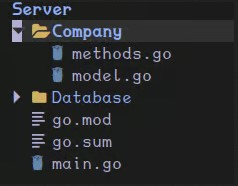
\includegraphics[width=5cm, height=4cm]{server.jpg}\\
\textit{Company} is a module. Our models.go file look like this:\\
\begin{lstlisting}[language=Go]
  package company
  import "github.com/google/uuid";
  type Company struct {
      Id string;
      Name string;
      Country string;
  }
  func newCompany(name string, country string) Company {
      return Company {
          Id: uuid.New().String(),
          Name: name,
          Country: country
      }
  }
\end{lstlisting}
Let's add a property \textit{manager} which is private. We cannot prevent the code of
the same module from accessing this property, however, we can prevent
other modules from accessing the property by making the first letter of the
name smallcase.
\begin{quotation}
  Names with the first letter as capital case are exported and the names
  with the first letter as small case are limited to the same module. This
  applies to properties, variables, types and functions. 
\end{quotation}
\break
\begin{lstlisting}[language=Go]
  type Company struct {
    Id string;
    Name string;
    Country string;
    manager string;
  }
\end{lstlisting}
\section*{Inheritance}
Although there is no direct concept of Inheritance in Go, we can embed base
structs into its child structs.\\
Let's say, we want to define \textit{Employee} struct also. Since it has the same
properties as the company we want it to inherit those properties from 
\textit{Company}. We can define it like this:
\begin{lstlisting}[language=Go]
  type Employee struct {
    Company;
    Salary int;
  }
\end{lstlisting}
To define function \textit{\textbf{newEmployee}}:
\begin{lstlisting}[language=Go]
  type newEmployee(companyName string, companyCountry string, salary int) Employee {
    company := newCompany(
      companyName,
      companyCountry
    )
    return Employee {
      Company: company,
      Salary: salary,
    }
  }
\end{lstlisting}
\begin{quote}
  Notice we used \textit{saveToDatabase} method of company with \textit{Employee} struct\\
  object.
\end{quote}
\section*{Polymorphism}
Go provides interfaces for this purpose. A type implementing a function or \\
multiple functions defined in the interface becomes the type of that\\
interface.\\
We will extend our current example and define another type of \\
VendorCompany. This is the company from which our current company buys\\
raw materials.\\
Implementation would be similar to Employee. Since all three of them are
similar objects and being saved into db in the same table/collection
(hypothetically), we would define an interface \textit{CompanyInterface} so that we
treat all three objects as the same type - the interface. Since we have also
defined three different types of entities into object, let's create a
method to return the type of entity when called.\\
\\model.go
\begin{lstlisting}[language=Go]
  package company
  import ("github.com/google/uuid")
  type CompanyInterface struct {
    saveToDatabase();
    getType() companyEntity;
  }
  type ComanyEnum string;
  const (
    CompanyType   CompanyEnum = "Company";
    VendorType    CompanyEnum = "Vendor";
    EmployeeType  CompanyEnum = "Employee";
  )
  type Company struct {
    Id string
    Name string
    Country string
    manager string
  }
  type Employee struct {
    Company
    Salary int
  }
  type VendorCompany struct {
    Company
    AccountNumber string
  }
  func newCompany(name string, country string) Company {
    return Company {
      Id: uuid.New().String(),
      Name: name,
      Country: country
    }
  }
  func newEmployee(companyName string, companyCountry string, salary int) {
    company := newCompany(companyName, companyCountry)
    employee := Employee {
      Company: company,
      Salary: salary
    }
    employee.saveToDatabase()
    return employee
  }
  func newVendor(companyName string, companyCountry string, accountNumber int) {
    company := newCompany(companyName, companyCountry)
    vendor := VendorCompany {
      Company: company,
      AccountNumber: accountNumber
    }
    vendor.saveToDatabase()
    return vendor
  }
\end{lstlisting}
methods.go
\begin{lstlisting}[language=Go]
  package company
  import "fmt"
  func(c *Company) saveToDatabase() {
    fmt.Println("Saving Company to database...")
  }
  func(c *Company) getType() CompanyEnum {
    return CompanyType
  }
  func(e *Employee) saveToDatabase() {
    fmt.Println("Saving Employee to database...")
  }
  func(e *Employee) getType() {
    return EmployeeType
  }
  func(v *VendorCompany) saveToDatabase() {
    fmt.Println("Saving VendorCompany to database...")
  }
  func(v *VendorCompany) getType() {
    return VendorType
  }
\end{lstlisting}
\end{document}